% graphicx
\documentclass[12pt, a4paper, onecolumn]{article}

% ---------- Packages ----------
\usepackage{graphicx} % .eps, .pdf, .png, .jpg, .jpeg
\usepackage{float}
\usepackage{caption}
\usepackage{subcaption}

\DeclareGraphicsExtensions{.pdf, .jpg, .png}

% \includegraphics[options]{image_path}
%                     ↓
% ---------------- Options ----------------
% 1- width = x
% 2- height = x
% 3- scale = [0-1]
% 4- keepaspectration = true/false
% 5- angle = x (degree)
% 6- trim = l b r t    % If you want to use it you must enable **clip** option
% 7- clip = true/false
% 8- page = x


% \begin{figure}[?]
%	             ↓
% \end{figure}   ↓
%                ↓
%--------------- ? ---------------
% 1- h	here
% 2- t	top
% 3- b	bottom
% 4- p	page
% 5- !	override
% 6- H	= h!	(must sue float package)

\begin{document}
	
	\begin{figure}[H]
		\centering
		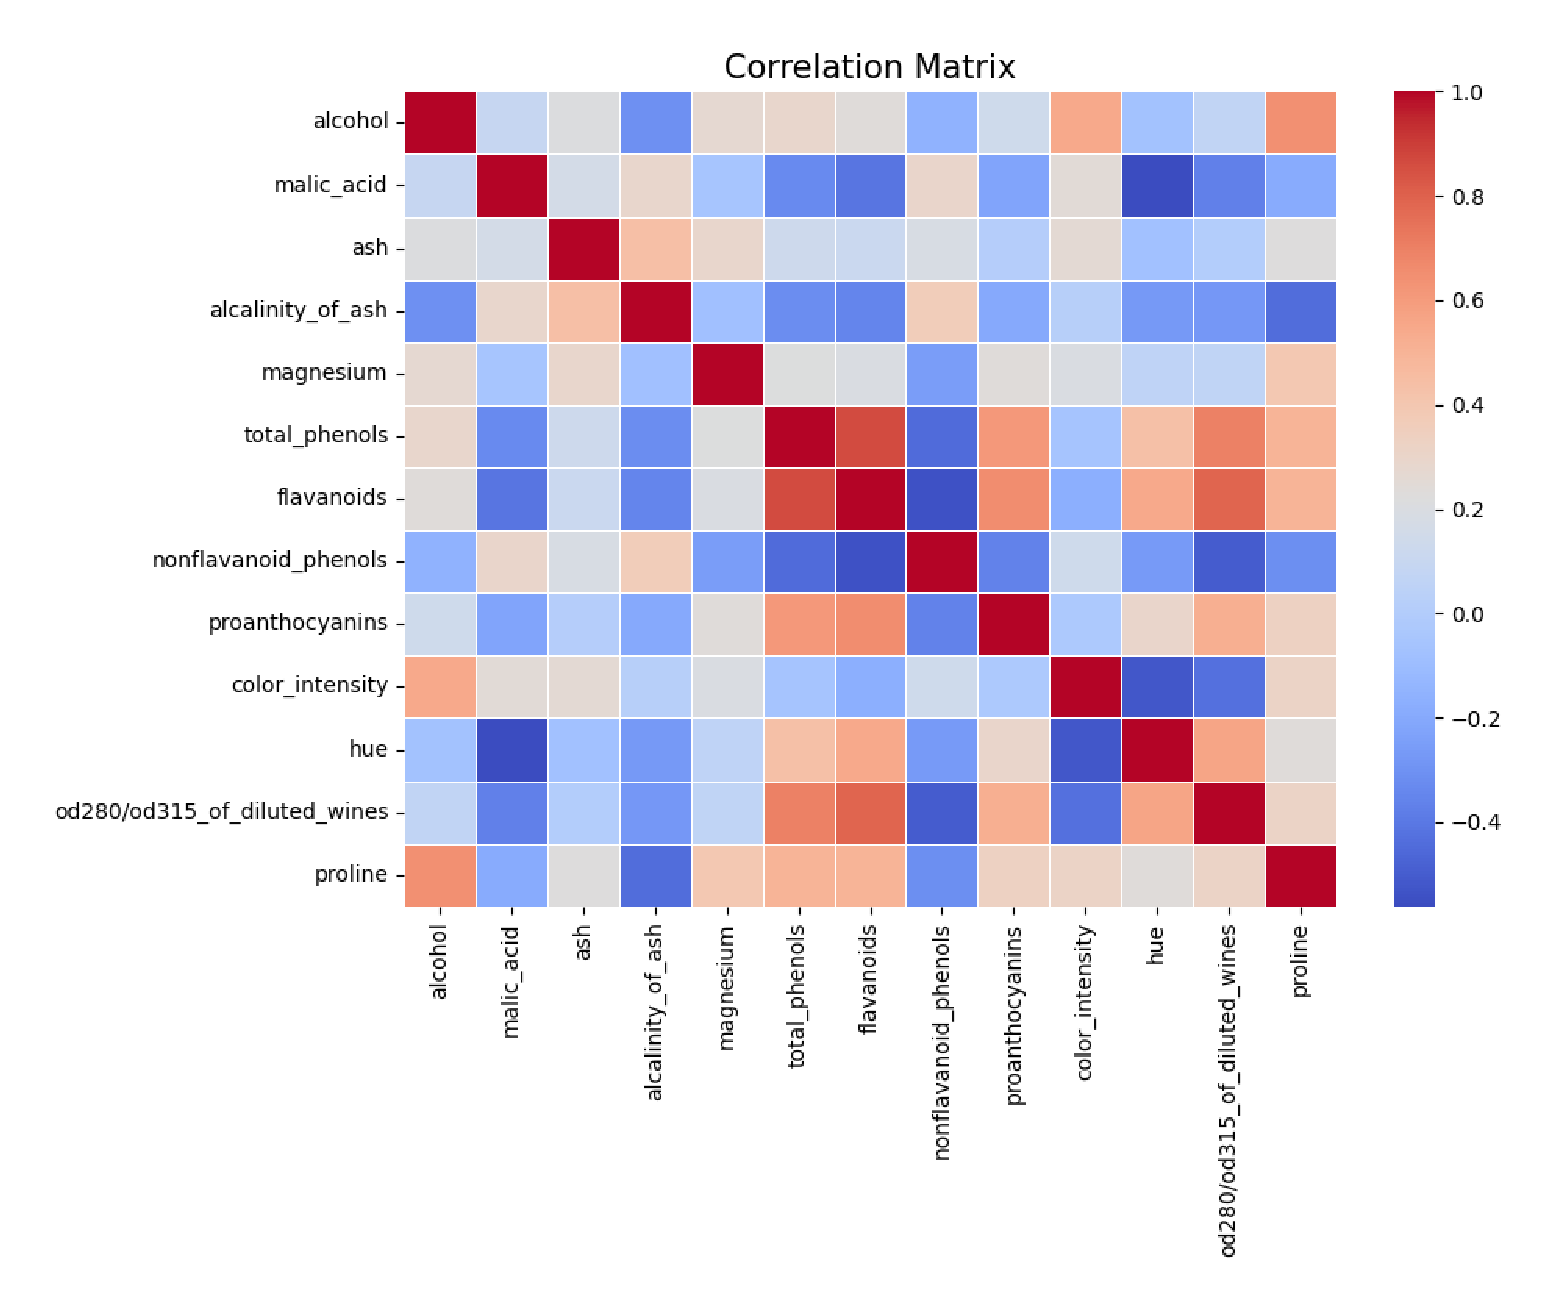
\includegraphics[width=0.7\textwidth]{img/pdf/correlation_matrix}
		\caption[Correlation Matrix]{Correlation Matrix of Wine Dataset}
		\label{fig:correlationmatrix}
	\end{figure}

	The plot of correlation matrix of wine Dataset is in Fig.\ref{fig:correlationmatrix}.
	
	\newpage
	% Subfigure:
	
	\begin{figure}
		\centering
		
		% Sub-fig 1
		\begin{subfigure}[b]{0.3\textwidth}
			\centering
			
\includegraphics[width=\textwidth]{img/jpg/gull}
			\caption[gull]{A gull}
			\label{subfig:gull}
		\end{subfigure}
		~
		% Sub-fig 2
		\begin{subfigure}[b]{0.3\textwidth}
			\centering
			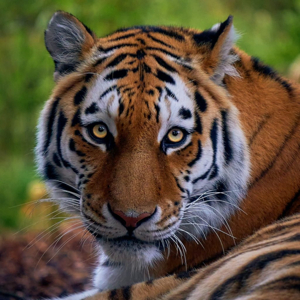
\includegraphics[width=\textwidth]{img/jpg/tiger}
			\caption[tiger]{A tiger}
			\label{subfig:tiger}
		\end{subfigure}
		~
		% Sub-fig 3
		\begin{subfigure}[b]{0.3\textwidth}
			\centering
			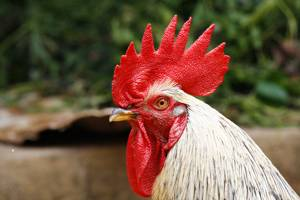
\includegraphics[width=1.41\textwidth, trim=20pt 0 0 0, clip=true]{img/jpg/rooster}
			\caption[rooster]{A rooster}
			\label{subfig:rooster}
		\end{subfigure}
		
		\caption[animals]{A group of animals}
		\label{fig:animals}
	\end{figure}
	

\end{document}